\documentclass{article}
\usepackage{sivaSAFRANshort}
\chead{Assignment $1$: Warmup}
\begin{document}
	\begin{enumerate}
		\item
		Prove that among all triangles with a fixed perimeter $P$, the equilateral triangle is the one that maximizes the area.
		\item
		Generalize the above for a $n$-sided polygon and prove it.
		\item
		Consider an acute angled triangle $ABC$ and a point $D$ on $BC$. Find points (by construction) $E$ on $AC$ and $F$ on $AB$ such that the perimeter of the triangle $DEF$ is minimum.
		\item
		Prove (via geometry) that the area of a cyclic quadrilateral is the maximum possible for any quadrilateral with given side lengths.
		\item
		\textbf{Bus terminus location problem}: Geometrically obtain the location of the bus terminus $T$ on the road segment $PQ$ such that the lengths of the roads linking $T$ with the two cities $A$ and $B$ is minimum.
		\begin{center}
		\begin{tikzpicture}
			\draw (0,0) -- (1,3);
			\draw [fill=cyan] (3,2) circle (0.1);
			\node at (3,2.375) {$B$};
			\draw [fill=cyan] (2,0.5) circle (0.1);
			\node at (2,0.875) {$A$};
			\draw [fill=red] (0.5,1.5) circle (0.1);
			\node at (0.125,1.5) {$T$};
		\end{tikzpicture}
		\end{center}
		\item
		Given two points $A$ and $B$ in a vertical plane (with $A$ above $B$), find the curve which the object must follow so that starting from $A$, it reaches $B$ in the shortest possible time under gravity.
		\begin{center}
		\begin{tikzpicture}
			\draw [fill=red] (0,0) circle (0.1);
			\draw [fill=red] (2,-1) circle (0.1);
			\draw [white] plot [smooth, tension=1] coordinates { (0,0) (0.5,-0.25) (1,-0.625) (1.5,-0.875) (2,-1)};
			\node at (-0.4,0) {$A$};
			\node at (2.4,-1) {$B$};
		\end{tikzpicture}
		\end{center}
		\item
		Given three cities $A$, $B$ and $C$, geometrically find the location where an artificial water reservoir must be constructed so that the sum of the length of the pipeline from the reservoir to the three cities is minimum.
		\item
		Prove the arithmetic mean geometric mean inequality, i.e.,
		$$\dfrac{a_1+a_2+\cdots+a_n}n \geq \sqrt[n]{a_1a_2\cdots a_n}$$
		where $a_i \geq 0$ and $n \in \Zb^+$.
		\item
		Prove that in any triangle $ABC$, we have
		$$\sin(A) + \sin(B) + \sin(C) \leq \dfrac{3\sqrt3}2$$
		\item
		It is desired to construct a bridge across a river so that the two cities, $A$ and $B$, on either side of the river are connected. Due to construction constraints it is desired to have the bridge to be perpendicular to the flow of the river. See Figure~\ref{bridge} for the details. Geometrically identify where the bridge needs to be located, i.e., the points $C$ and $D$, so that the distance of the path from $A$ to $B$ is minimized.
		\begin{figure}[!htbp]
			\begin{center}
			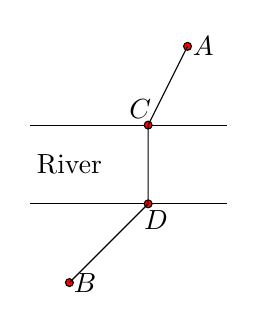
\begin{tikzpicture}[scale=0.5]
				\draw (0,0) -- (5,0);
				\draw (0,-2) -- (5,-2);
				\draw [fill=red] (4,2) circle (0.1);
				\draw [fill=red] (1,-4) circle (0.1);
				\draw [fill=red] (3,0) circle (0.1);
				\draw [fill=red] (3,-2) circle (0.1);
				\draw (4,2) -- (3,0) -- (3,-2) -- (1,-4);
				\node at (4.4,2) {$A$};
				\node at (1.4,-4) {$B$};
				\node at (2.8,0.4) {$C$};
				\node at (3.2,-2.4) {$D$};
				\node at (1,-1) {River};
			\end{tikzpicture}
			\caption{Bridge construction}
			\label{bridge}
			\end{center}
		\end{figure}
	\end{enumerate}
\end{document}